% vim: ft=tex
\chapter{Project monitoring}
\section{Performance analysis}
\subsection{Weekly overview}

\autoref{fig:projmon:weekly} illustrates the weekly time spent on this bachelor
thesis. The thick horizontal line represents the planned effort of 28.5 hours a
week, which has been calculated using the risk analysis explained
in~\autoref{sec:projplan:est-time}.  Milestones are denoted by the green
labels. The legend along the x-axis represents the semester weeks, including
the particular RUP phases.


\begin{figure}
	% TODO Fillup the right data
	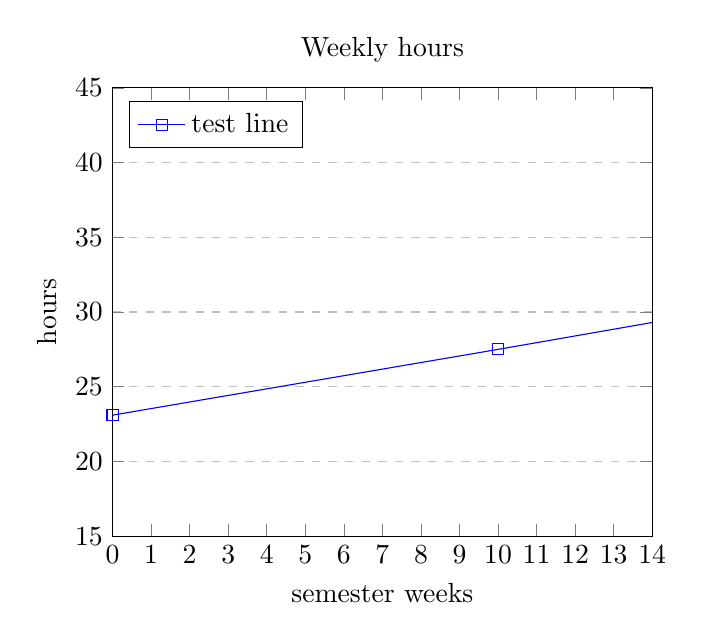
\begin{tikzpicture}
	\begin{axis}[
	    title={Weekly hours},
	    xlabel={semester weeks},
	    ylabel={hours},
	    xmin=0, xmax=14,
	    ymin=15, ymax=45,
	    xtick={0,1,2,3,4,5,6,7,8,9,10,11,12,13,14},
	    ytick={0,5,10,15,20,25,30,35,40,45},
	    legend pos=north west,
	    ymajorgrids=true,
	    grid style=dashed,
	]
	 
	\addplot[
	    color=blue,
	    mark=square,
	    ]
	    coordinates {
	    (0,23.1)(10,27.5)(20,32)(30,37.8)(40,44.6)(60,61.8)(80,83.8)(100,114)
	    };
	    \legend{test line}
	 
	\end{axis}
	\end{tikzpicture}
	\caption{Weekly performance analysis}
	\label{fig:projmon:weekly}
\end{figure}

% TODO Translate
Wie man aus dieser Grafik herauslesen kann, haben wir zu Beginn der Arbeit 
am wenigsten Stunden pro Woche aufgewendet. Das liegt daran, dass wir zuerst die 
genauen Anforderungen abklären mussten und teilweise erst nach einer Besprechung 
oder einer Rückmeldung an bestimmten Punkten weiterarbeiten konnten. 
Vor dem Meilenstein „Release“ hatten wir alle Informationen zusammen und 
konnten mit vollem Elan die Anforderungen umsetzen.

\subsection{Overall overview}
% TODO Fillup the right data
\begin{tikzpicture}
\begin{axis}[
	title={total hours - project},
	x tick label style={
		/pgf/number format/1000 sep=},
	ylabel=Hours,
	enlargelimits=0.05,
	legend style={at={(0.5,-0.1)},
	anchor=north,legend columns=-1},
	ybar interval=0.7,
]
\addplot 
	coordinates {(1, 720)};
\addplot 
	coordinates {(2, 800)};
\legend{should, is}
\end{axis}
\end{tikzpicture}

% TODO translate
In dieser Abbildung wird ersichtlich, dass wir die, von der Modulbeschreibung geforderten, 
Soll-Stunden um 10% überschritten haben. Der Grund der Überschreitung ist unteranderem
die Implementation des optionalen Features und die grossflächig angelegten Tests.

% TODO Fillup the right data
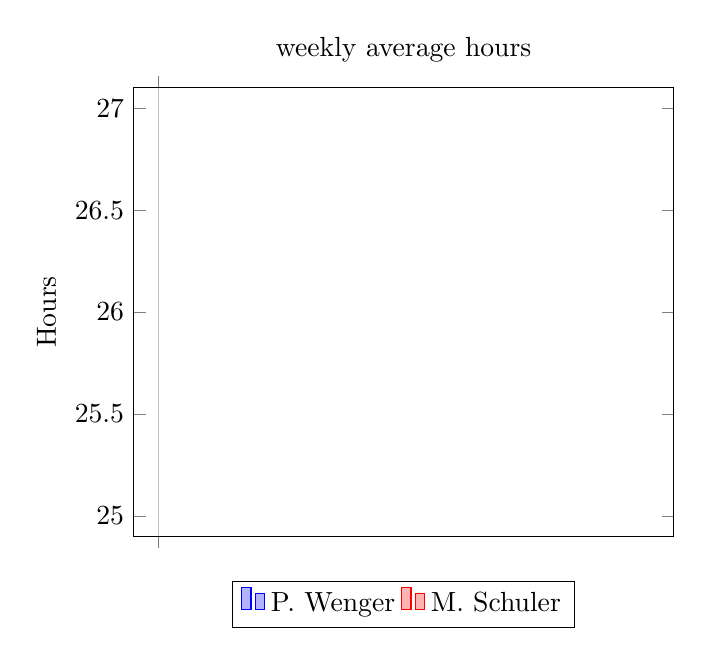
\begin{tikzpicture}
\begin{axis}[
	title={weekly average hours},
	x tick label style={
		/pgf/number format/1000 sep=},
	ylabel=Hours,
	enlargelimits=0.05,
	legend style={at={(0.5,-0.1)},
	anchor=north,legend columns=-1},
	ybar interval=0.7,
]
\addplot 
	coordinates {(1, 27)};
\addplot 
	coordinates {(2, 25)};
\legend{P. Wenger, M. Schuler}
\end{axis}
\end{tikzpicture}

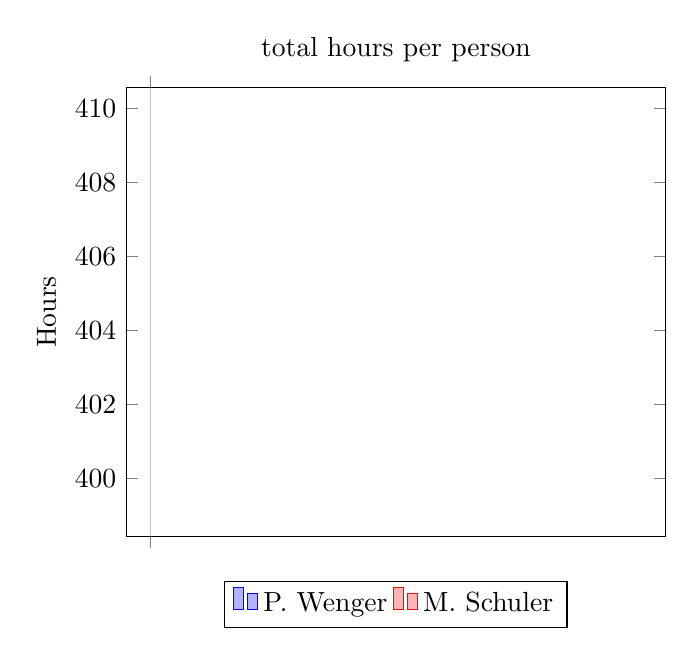
\begin{tikzpicture}
\begin{axis}[
	title={total hours per person},
	x tick label style={
		/pgf/number format/1000 sep=},
	ylabel=Hours,
	enlargelimits=0.05,
	legend style={at={(0.5,-0.1)},
	anchor=north,legend columns=-1},
	ybar interval=0.7,
]
\addplot 
	coordinates {(1, 410)};
\addplot 
	coordinates {(2, 399)};
\legend{P. Wenger, M. Schuler}
\end{axis}
\end{tikzpicture}


% TODO translate
Die einzelnen Personen haben ein sehr ausgeglichenes Stundentotal. 
Das liegt daran, dass wir in regelmässigen Abständen eine Auswertung 
in Everhour gemacht haben und dadurch die Tasks gerechter verteilen konnten. 

Die Archivdaten unseres Everhour Projekts befinden sich auf dem Moodle. 
In diesem kann detailliert nachverfolgt werden, 
für welche Tasks wir wie viel Zeit aufgewendet haben.


\subsection{Aufgewendete Stunden nach Feature}
% TODO Translate
Da wir in dieser Arbeit ein bestehendes Produkt erweitert haben war es zu beginn an
schwierig die Aufwände abzuschätzen. Die Soll/Ist Abschätzungen wurden von Iteration zu Iteration
immer genauer. Nachfolgend die Soll/Ist Aufwandschätzung der einzelnen Feature.

% TODO Fillup the right data
\begin{tikzpicture}
\begin{axis}[
	title={hours per feature},
	x tick label style={
		/pgf/number format/1000 sep=},
	ylabel=Hours,
	enlargelimits=0.05,
	legend style={at={(0.5,-0.1)},
	anchor=north,legend columns=-1},
	ybar interval=0.7,
]
\addplot 
	coordinates {(1, 50)};
\addplot 
	coordinates {(2, 40)};
\legend{is, should}
\end{axis}
\end{tikzpicture}
